\pdfbookmark{Общая характеристика работы}{characteristic}             % Закладка pdf
\section*{\centering ОБЩАЯ ХАРАКТЕРИСТИКА РАБОТЫ}

\newcommand{\actuality}{\pdfbookmark[1]{Актуальность}{actuality}\textit{\actualityTXT}}
\newcommand{\progress}{\pdfbookmark[1]{Разработанность темы}{progress}\textit{\progressTXT}}
\newcommand{\aim}{\pdfbookmark[1]{Цели}{aim}{\textit\aimTXT}}
\newcommand{\tasks}{\pdfbookmark[1]{Задачи}{tasks}\textit{\tasksTXT}}
\newcommand{\theoretical}{\pdfbookmark[1]{Теоретическая значимость}{theoretical}\textit{\theoreticalTXT}} % Added by ASM
\newcommand{\aimtasks}{\pdfbookmark[1]{Цели и задачи}{aimtasks}\aimtasksTXT}
\newcommand{\researchobj}{\pdfbookmark[1]{Объект исследования}{researchobj}\textit{\researchobjTXT}}
\newcommand{\researchsubj}{\pdfbookmark[1]{Предмет исследования}{researchsubj}\textit{\researchsubjTXT}}
\newcommand{\novelty}{\pdfbookmark[1]{Научная новизна}{novelty}\textit{\noveltyTXT}}
\newcommand{\influence}{\pdfbookmark[1]{Практическая значимость}{influence}\textit{\influenceTXT}}
\newcommand{\methods}{\pdfbookmark[1]{Методология и методы исследования}{methods}\textit{\methodsTXT}}
\newcommand{\defpositions}{\pdfbookmark[1]{Положения, выносимые на защиту}{defpositions}\textit{\defpositionsTXT}}
\newcommand{\pasport}{\pdfbookmark[1]{Соответствие паспорту научной специальности}{pasport}\textit{\pasportTXT}} % Почему этого здесь не было?
\newcommand{\reliability}{\pdfbookmark[1]{Достоверность}{reliability}\textit{\reliabilityTXT}}
\newcommand{\probation}{\pdfbookmark[1]{Апробация результатов}{probation}\textit{\probationTXT}}
%\newcommand{\reliaprobation}{\pdfbookmark[1]{Достоверность и Апробация}{reliaprobation}\textit{\reliaprobationTXT}} % Вместо Достоверности и Апробации вместе...
\newcommand{\contribution}{\pdfbookmark[1]{Личный вклад}{contribution}\textit{\contributionTXT}}%}
\newcommand{\publications}{\pdfbookmark[1]{Публикации}{publications}\textit{\publicationsTXT}}%}

\input{common/characteristic} % Характеристика работы по структуре во введении и в автореферате не отличается (ГОСТ Р 7.0.11, пункты 5.3.1 и 9.2.1), потому её загружаем из одного и того же внешнего файла, предварительно задав форму выделения некоторым параметрам

%Диссертационная работа была выполнена при поддержке грантов \dots

%\underline{\textbf{Объем и структура работы.}} Диссертация состоит из~введения,
%четырех глав, заключения и~приложения. Полный объем диссертации
%\textbf{ХХХ}~страниц текста с~\textbf{ХХ}~рисунками и~5~таблицами. Список
%литературы содержит \textbf{ХХX}~наименование.

\textit{Структура диссертации}. %}:  
%\ref*{disTotPages}
%\formbytotal{dis_totalchapter}{глав}{ы}{}{},
%\formbytotal{\ref*{distotalappendix}}{приложен}{ия}{ий}{ий}.
%% на случай ошибок оставляю исходный кусок на месте, закомментированным
%Полный объём диссертации составляет  \ref*{TotPages}~страницу
%с~\totalfigures{}~рисунками и~\totaltables{}~таблицами. Список литературы
%содержит \total{citenum}~наименований.
Общий объём диссертации составляет \ref*{disTotPages} страниц машинописного текста. Диссертация
состоит из~введения, 4 разделов, 
%\ref*{disTotPages}
%\formbytotal{dis_totalchapter}{глав}{ы}{}{},
заключения, списка литературы, включающего 76 наименований, содержит
52 таблицы, 43 рисунка и 3 приложения. 

%\formbytotal{\ref*{disTotPages}}{страниц}{у}{ы}{}, включая
%\formbytotal{\ref*{distotalcount@figure}}{рисун}{ок}{ка}{ков} и
%\formbytotal{distotalcount@table}{таблиц}{у}{ы}{}.
%Список литературы содержит
%\formbytotal{discitenum}{наименован}{ие}{ия}{ий}.



\newpage

\pdfbookmark{Содержание работы}{description}                          % Закладка pdf
\section*{Содержание работы}
% ВВЕДЕНИЕ
Во \textit{введении} обосновывается актуальность исследований, проводимых в~рамках данной диссертационной работы. Сформированы цели и задачи диссертационного исследования. Представлены научные положения, выносимые на защиту.

\medskip
% Глава 1
В \textit{первом разделе} проведен теоретических анализ
факторов, влияющих на точность передачи координат с использованием спутниковых методов. Помимо этого, приводится классификация РРР-способов обработки спутниковых данных.

\input{Dissertation/part1}

\medskip
% Глава 2
Во \textit{втором разделе} диссертационной работы рассмотрены современные методы обработки спутниковых измерений по РРР-алгоритму. 
\input{Dissertation/part2}

\medskip
%Глава3
\textit{Третий раздел} посвящен разработке методики создания геодезических сетей при использовании РРР-алгоритма обработки спутниковых данных.

\input{Dissertation/part3}

\medskip
% Глава 4

\begin{minipage}[b][.5cm][b]{0.9\linewidth}
	~
\end{minipage}
В \textit{четвёртой главе} приведены результаты применения предложенной методики для сетей, построенных, в диапазоне расстояний: от~700 до~1000~км; от~1000 до~1300~км; от~1300 до~1700~км.

\chapter{ИССЛЕДОВАНИЕ ТОЧНОСТИ ПОСТРОЕНИЯ ГЕОДЕЗИЧЕСКИХ СЕТЕЙ ПРИ УРАВНИВАНИИ СЕТЕЙ В ДИАПАЗОНАХ
	РАССТОЯНИЙ ОТ~700 ДО 1600~КМ}\label{ch:ch4}

\section{Исследование точности при построении геодезической сети в диапазоне расстояний от~700 до 1000~км}\label{sec:ch4/sect1}

На рисунке \cref{fig:pic41} приведена схема создаваемой сети при использовании РРР-алгоритма. В качестве исходных данных были получены RINEX-файлы с пунктов сети базовых станций EFT~COORS.


\begin{figure}[!h]
	\centering
	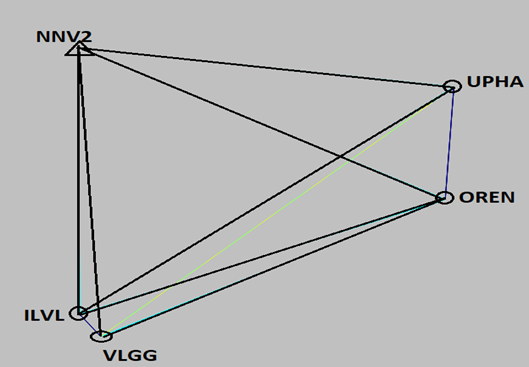
\includegraphics[width=0.99\linewidth]{images/pic41}
	\caption{Cхема сети }
	\label{fig:pic41}
\end{figure}


Геодезическая сеть состоит из пяти пунктов, равномерно расположенных в диапазоне расстояний от~$700$ до $1000$~км. Среднее расстояние между пунктами --- $850$~км.

Как и прежде, происходила обработка RINEX файлов с использованием интернет-сервиса CSRS. Для контроля получаемой точности выполнена обработка в программном обеспечении Trimble Business Centre (далее «TBC») и в статике с использованием ПО~«КРЕДО ГНСС». В последствии получены вектора и выполнено уравнивание с оценкой точности, результаты которой приведены в таблице \cref{tab:tab59}.


\begin{table} [htbp]
	\centering\small
	\begin{threeparttable}% выравнивание подписи по границам таблицы
		\captionof{table}{Оценка точности при уравнивании}\label{tab:tab59}
		\setlength{\tabcolsep}{15pt}
		\sisetup{
			table-figures-integer = 3
		}{
			\begin{tabular}{lcccccc}
				\toprule %\hline
				\textbf{~}	& \multicolumn{2}{c}{ \textbf{RTX-TBC} }	& \multicolumn{2}{c}{ \textbf{CRSR} }	& \multicolumn{2}{c}{ \textbf{статика кредо} }	\\ %\hline
				\textbf{Интервал}	& 	$\mathbf{m_{xy}}$\textbf{, м}	& $\mathbf{m_{z}}$\textbf{, м}	&
							  			$\mathbf{m_{xy}}$\textbf{, м}	& $\mathbf{m_{z}}$\textbf{, м}	& 
							  			$\mathbf{m_{xy}}$\textbf{, м}	& $\mathbf{m_{z}}$\textbf{, м}	\\ %\hline
				\midrule
				$\mathbf{1}$~ч.	& $0,023$	& $0,032$	& $0,021$	& $0,029$	& $0,095$	& $0,119$	\\ %\hline
				$\mathbf{2}$~ч.	& $0,022$	& $0,031$	& $0,019$	& $0,027$	& $0,093$	& $0,115$	\\ %\hline
				$\mathbf{3}$~ч.	& $0,021$	& $0,030$	& $0,018$	& $0,026$	& $0,089$	& $0,102$	\\ %\hline
				$\mathbf{4}$~ч.	& $0,021$	& $0,030$	& $0,018$	& $0,026$	& $0,086$	& $0,097$	\\ %\hline
				
				\bottomrule
			\end{tabular}
		}
	\end{threeparttable}
\end{table}

Как видно из таблицы \cref{tab:tab59} точность определения по РРР-алгоритму сопоставима между собой и несколько превосходит точность, получаемую в статике.



\section{Исследование точности при построении геодезической сети в диапазоне расстояний от~1000 до 1300~км}\label{sec:ch4/sect2}

На рисунке \cref{fig:pic42} приведена схема создаваемой сети при использовании РРР-алгоритма. В качестве исходных данных были получены RINEX-файлы с пунктов сети базовых станций EFT COORS.


\begin{figure}[!h]
	\centering
	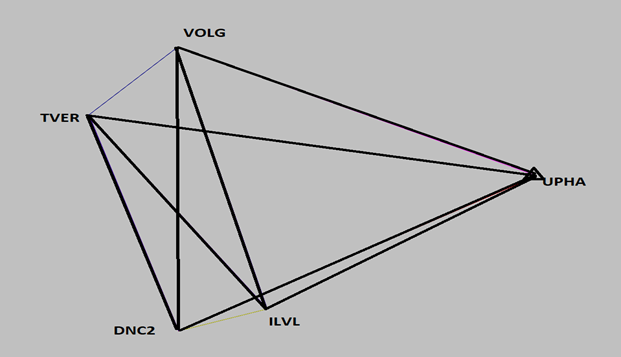
\includegraphics[width=0.99\linewidth]{images/pic42}
	\caption{Cхема сети }
	\label{fig:pic42}
\end{figure}

Геодезическая сеть состоит из пяти пунктов, равномерно расположенных в диапазоне расстояний от~$1000$ до $1300$~км. В рамках сети происходит определение восьми векторов. Для выполнения работ требуется два сеанса измерений для обеспечения их независимости.

Как и прежде, происходила обработка RINEX файлов с использованием интернет-сервиса CSRS. Для контроля получаемой точности выполнена обработка в программном обеспечении TBC и в статике с использованием ПО~«КРЕДО ГНСС». Подробнее с процессами обработки можно ознакомиться [$\ldots$]. В таблице \cref{tab:tab60} приводится оценка точности.


\begin{table} [htbp]
	\centering\small
	\begin{threeparttable}% выравнивание подписи по границам таблицы
		\captionof{table}{Оценка точности при уравнивании}\label{tab:tab60}
		\setlength{\tabcolsep}{15pt}
		\sisetup{
			table-figures-integer = 3
		}{
			\begin{tabular}{lcccccc}
				\toprule %\hline
				\textbf{~}	& \multicolumn{2}{c}{ \textbf{RTX-TBC} }	& \multicolumn{2}{c}{ \textbf{CRSR} }	& \multicolumn{2}{c}{ \textbf{статика кредо} }	\\ %\hline
				\textbf{Интервал}	& 	$\mathbf{m_{xy}}$\textbf{, м}	& $\mathbf{m_{z}}$\textbf{, м}	&
				$\mathbf{m_{xy}}$\textbf{, м}	& $\mathbf{m_{z}}$\textbf{, м}	& 
				$\mathbf{m_{xy}}$\textbf{, м}	& $\mathbf{m_{z}}$\textbf{, м}	\\ %\hline
				\midrule
				$\mathbf{1}$~ч.	& $0,040$	& $0,041$	& $0,040$	& $0,042$	& $0,252$	& $0,407$	\\ %\hline
				$\mathbf{2}$~ч.	& $0,037$	& $0,038$	& $0,039$	& $0,039$	& $0,243$	& $0,337$	\\ %\hline
				$\mathbf{3}$~ч.	& $0,036$	& $0,038$	& $0,037$	& $0,038$	& $0,196$	& $0,290$	\\ %\hline
				$\mathbf{4}$~ч.	& $0,033$	& $0,037$	& $0,037$	& $0,038$	& $0,185$	& $0,246$	\\ %\hline
				
				\bottomrule
			\end{tabular}
		}
	\end{threeparttable}
\end{table}

Как видно из таблицы \cref{tab:tab60} точность при уравнивании по РРР-алгоритму, по-прежнему, сопоставима между собой и на порядок выше, чем при классической обработке в статике.




\section{Исследование точности при построении геодезической сети в диапазоне расстояний от~1300 до 1700~км}\label{sec:ch4/sect3}

На рисунке \cref{fig:pic43} приведена схема создаваемой сети при использовании РРР-алгоритма. В качестве исходных данных были получены RINEX-файлы с пунктов сети базовых станций EFT COORS.


\begin{figure}[!h]
	\centering
	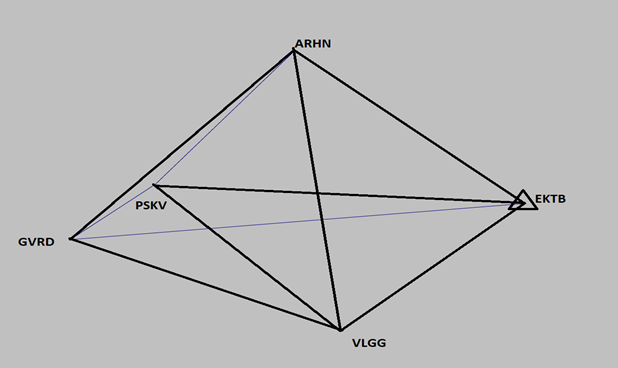
\includegraphics[width=0.99\linewidth]{images/pic43}
	\caption{Cхема сети }
	\label{fig:pic43}
\end{figure}

Геодезическая сеть состоит из пяти пунктов, равномерно расположенных в диапазоне расстояний от~$1\mathbf{4}00$ до $1900$~км. 
\footnote{Так до какого, всётаки расстояния? 1700~км, как в заголовке раздела? Или 1600~км, как в заголовке Главы? Или 1900~км, здесь? ;) }
В рамках сети происходит определение восьми векторов. Для выполнения работ требуется два сеанса измерений для обеспечения их независимости.

Как и прежде, происходила обработка RINEX файлов с использованием интернет-сервиса CSRS. Для контроля получаемой точности выполнена обработка в программном обеспечении TBC и в статике с использованием ПО~«КРЕДО ГНСС». Подробнее с процессами обработки можно ознакомиться [$\ldots$]. В таблице \cref{tab:tab61} приводится оценка точности.


\begin{table} [htbp]
	\centering\small
	\begin{threeparttable}% выравнивание подписи по границам таблицы
		\captionof{table}{Оценка точности при уравнивании}\label{tab:tab61}
		\setlength{\tabcolsep}{15pt}
		\sisetup{
			table-figures-integer = 3
		}{
			\begin{tabular}{lcccccc}
				\toprule %\hline
				\textbf{~}	& \multicolumn{2}{c}{ \textbf{RTX-TBC} }	& \multicolumn{2}{c}{ \textbf{CRSR} }	& \multicolumn{2}{c}{ \textbf{статика кредо} }	\\ %\hline
				\textbf{Интервал}	& 	$\mathbf{m_{xy}}$\textbf{, м}	& $\mathbf{m_{z}}$\textbf{, м}	&
				$\mathbf{m_{xy}}$\textbf{, м}	& $\mathbf{m_{z}}$\textbf{, м}	& 
				$\mathbf{m_{xy}}$\textbf{, м}	& $\mathbf{m_{z}}$\textbf{, м}	\\ %\hline
				\midrule
				$\mathbf{1}$~ч.	& $0,048$	& $0,051$	& $0,049$	& $0,052$	& $0,402$	& $0,290$	\\ %\hline
				$\mathbf{2}$~ч.	& $0,047$	& $0,050$	& $0,048$	& $0,049$	& $0,368$	& $0,263$	\\ %\hline
				$\mathbf{3}$~ч.	& $0,046$	& $0,049$	& $0,047$	& $0,048$	& $0,335$	& $0,242$	\\ %\hline
				$\mathbf{4}$~ч.	& $0,046$	& $0,049$	& $\mathbf{0,037} - ?$	& $0,048$	& $0,290$	& $0,215$	\\ %\hline
				
				\bottomrule
			\end{tabular}
		}
	\end{threeparttable}
\end{table}

Как видно из таблицы \cref{tab:tab61} точность при уравнивании по РРР-алгоритму, по-прежнему, сопоставима между собой и на порядок выше, чем при классической обработке в статике.




\FloatBarrier

\pagebreak%
% ЗАКЛЮЧЕНИЕ
\pdfbookmark{Заключение}{conclusion}          % Закладка pdf
\begin{minipage}[b][2.5cm][b]{5cm}
\section*{Заключение}
\end{minipage}

%\chapter*{Заключение}                       % Заголовок
\addcontentsline{toc}{chapter}{Заключение}  % Добавляем его в оглавление

%% Согласно ГОСТ Р 7.0.11-2011:
%% 5.3.3 В заключении диссертации излагают итоги выполненного исследования, рекомендации, перспективы дальнейшей разработки темы.
%% 9.2.3 В заключении автореферата диссертации излагают итоги данного исследования, рекомендации и перспективы дальнейшей разработки темы.
%% Поэтому имеет смысл сделать эту часть общей и загрузить из одного файла в автореферат и в диссертацию:

Итогом выполнения диссертационной работы на соискание ученой степени кандидата технических наук является разработанная методика по созданию геодезических сетей при использовании РРР-алгоритма обработки спутниковых данных.

Основные научные и практические результаты заключаются в решении следующих актуальных научных задач:

%% Согласно ГОСТ Р 7.0.11-2011:
%% 5.3.3 В заключении диссертации излагают итоги выполненного исследования, рекомендации, перспективы дальнейшей разработки темы.
%% 9.2.3 В заключении автореферата диссертации излагают итоги данного исследования, рекомендации и перспективы дальнейшей разработки темы.
Итогом выполнения диссертационной работы на соискание ученой степени кандидата технических наук, выполненной с целью совершенствования методики передачи координат в широком диапазоне расстояний при использовании современных методов обработки спутниковых данных, а также исследование различных факторов, влияющих на точность определения координат по РРР-алгоритму, является разработанная методика по созданию геодезических сетей при использовании РРР-алгоритма обработки спутниковых данных.

Основные научные и практические результаты заключаются в решении следующих актуальных научно-технических задач:

\begin{enumerate}
	\item Выполнено теоретическое и экспериментальное обоснование возможности использования РРР-алгоритма для построения геодезических сетей в различных диапазонах расстояний, которое позволило.......
	\item Проведены теоретические и экспериментальные исследования с целью выбора оптимальных параметров для обработки данных по РРР-алгоритму, которые позволили..........
	\item выполненные теоретические и экспериментальные исследования с целью выявления факторов, влияющих на точность обработки данных по РРР-алгоритму.
	
%	информационно-аналитический обзоров существующих методов создания геодезических сетей с использованием спутниковой аппаратуры. Приводятся основные требования по созданию геодезических сетей на примере ВГС (высокоточной геодезической сети) и СГС-1 (спутниковой геодезической сети).
%	\item Проведено научное исследование по выявлению влияния факторов на точность обработки данных по РРР-алгоритму. В качестве оцениваемых факторов были выделены следующие: продолжительность измерений; количество используемых спутников в процессе обработки по РРР-алгоритму; конфигурации различных ГНСС; влияние pdop фактора на точность; влияние дискретности (частоты записи).
%	\item Разработана методика создания геодезических сетей с использованием РРР-алгоритма обработки спутниковых данных. Методику можно применять при построении геодезических сетей, в том числе государственной геодезической сети. В ходе экспериментальных исследований было установлено, что точность определения координат с использованием РРР-алгоритма получается несколько выше, чем при классической обработке в статике.
\end{enumerate}
%
%	\item Теоретическое и экспериментальное обоснование возможности использования РРР-алгоритма для построения геодезических сетей в различных диапазонах расстояний.
%	\item Теоретические и экспериментальные исследования с целью выбора оптимальных параметров для обработки данных по РРР-алгоритму.
%	\item Теоретические и экспериментальные исследования с целью выявления факторов, влияющих на точность обработки данных по РРР-алгоритму.

Результаты диссертационного исследования рекомендуются к использованию при поддержании и развитии ГГС, а также для дальнейшего исследования точностных возможностей определения координат при использовании РРР-алгоритма.

Перспективы дальнейших исследований по данному направлению заключаются .......





Результаты диссертационного исследования рекомендуются к использованию при поддержании и развитии ГГС, а также для дальнейшего исследования точностных возможностей определения координат при использовании РРР-алгоритма.

Основные рекомендации по необходимости развития геодезических сетей, в том числе государственной геодезической сети включены в отчет НИР Министерства Сельского Хозяйства РФ по теме, выполненной в 2022 году.

Помимо этого, основные результаты исследования построения геодезических сетей при использовании РРР-алгоритма обработки спутниковых данных включены в отчеты по выполнению госбюджетной НИР кафедры
«Геодезия, геоинформатика и навигация» Российского Университета Транспорта, РУТ(МИИТ) за период 2021-2022 года. А также \textbf{будут ?} включены в отчет по госбюджетной НИР за период 2023-2024 годы.






\dotfill

Последний параграф может включать благодарности.  В заключение автор
выражает благодарность и большую признательность научному руководителю
Иванову~И.\,И. за поддержку, помощь, обсуждение результатов и~научное
руководство. Также автор благодарит Сидорова~А.\,А. и~Петрова~Б.\,Б.
за помощь в~работе с~образцами, Рабиновича~В.\,В. за предоставленные
образцы и~обсуждение результатов, Занудятину~Г.\,Г. и авторов шаблона
*Russian-Phd-LaTeX-Dissertation-Template* за~помощь в оформлении
диссертации. Автор также благодарит много разных людей
и~всех, кто сделал настоящую работу автора возможной.

%% Согласно ГОСТ Р 7.0.11-2011:
%% 5.3.3 В заключении диссертации излагают итоги выполненного исследования, рекомендации, перспективы дальнейшей разработки темы.
%% 9.2.3 В заключении автореферата диссертации излагают итоги данного исследования, рекомендации и перспективы дальнейшей разработки темы.
Итогом выполнения диссертационной работы на соискание ученой степени кандидата технических наук, выполненной с целью совершенствования методики передачи координат в широком диапазоне расстояний при использовании современных методов обработки спутниковых данных, а также исследование различных факторов, влияющих на точность определения координат по РРР-алгоритму, является разработанная методика по созданию геодезических сетей при использовании РРР-алгоритма обработки спутниковых данных.

Основные научные и практические результаты заключаются в решении следующих актуальных научно-технических задач:

\begin{enumerate}
	\item Выполнено теоретическое и экспериментальное обоснование возможности использования РРР-алгоритма для построения геодезических сетей в различных диапазонах расстояний, которое позволило.......
	\item Проведены теоретические и экспериментальные исследования с целью выбора оптимальных параметров для обработки данных по РРР-алгоритму, которые позволили..........
	\item выполненные теоретические и экспериментальные исследования с целью выявления факторов, влияющих на точность обработки данных по РРР-алгоритму.
	
%	информационно-аналитический обзоров существующих методов создания геодезических сетей с использованием спутниковой аппаратуры. Приводятся основные требования по созданию геодезических сетей на примере ВГС (высокоточной геодезической сети) и СГС-1 (спутниковой геодезической сети).
%	\item Проведено научное исследование по выявлению влияния факторов на точность обработки данных по РРР-алгоритму. В качестве оцениваемых факторов были выделены следующие: продолжительность измерений; количество используемых спутников в процессе обработки по РРР-алгоритму; конфигурации различных ГНСС; влияние pdop фактора на точность; влияние дискретности (частоты записи).
%	\item Разработана методика создания геодезических сетей с использованием РРР-алгоритма обработки спутниковых данных. Методику можно применять при построении геодезических сетей, в том числе государственной геодезической сети. В ходе экспериментальных исследований было установлено, что точность определения координат с использованием РРР-алгоритма получается несколько выше, чем при классической обработке в статике.
\end{enumerate}
%
%	\item Теоретическое и экспериментальное обоснование возможности использования РРР-алгоритма для построения геодезических сетей в различных диапазонах расстояний.
%	\item Теоретические и экспериментальные исследования с целью выбора оптимальных параметров для обработки данных по РРР-алгоритму.
%	\item Теоретические и экспериментальные исследования с целью выявления факторов, влияющих на точность обработки данных по РРР-алгоритму.

Результаты диссертационного исследования рекомендуются к использованию при поддержании и развитии ГГС, а также для дальнейшего исследования точностных возможностей определения координат при использовании РРР-алгоритма.

Перспективы дальнейших исследований по данному направлению заключаются .......





\newpage



\pdfbookmark{Литература}{bibliography}                                % Закладка pdf


\ifdefmacro{\microtypesetup}{\microtypesetup{protrusion=false}}{} % не рекомендуется применять пакет микротипографики к автоматически генерируемому списку литературы
\urlstyle{rm}                               % ссылки URL обычным шрифтом
\ifnumequal{\value{bibliosel}}{0}{% Встроенная реализация с загрузкой файла через движок bibtex8
    \renewcommand{\bibname}{\large \bibtitleauthor}
    \nocite{*}
    \insertbiblioauthor           % Подключаем Bib-базы
    %\insertbiblioexternal   % !!! bibtex не умеет работать с несколькими библиографиями !!!
}{% Реализация пакетом biblatex через движок biber
    % Цитирования.
    %  * Порядок перечисления определяет порядок в библиографии (только внутри подраздела, если `\insertbiblioauthorgrouped`).
    %  * Если не соблюдать порядок "как для \printbibliography", нумерация в `\insertbiblioauthor` будет кривой.
    %  * Если цитировать каждый источник отдельной командой --- найти некоторые ошибки будет проще.
    %
    %% authorvak
    \nocite{mak02}%
    \nocite{mak06}%
    \nocite{mak07}%
    \nocite{mak08}%
    \nocite{mak11}%
%    \nocite{mak0}%
    %
    %% authorwos
%    \nocite{wosbib1}%
    %
    %% authorscopus
%    \nocite{scbib1}%
    %
    %% authorpathent
%    \nocite{patbib1}%
    %
    %% authorprogram
%    \nocite{progbib1}%
    %
    %% authorconf
    \nocite{mak01}%
    \nocite{mak03}%
    \nocite{mak04}%
    \nocite{mak05}%
    \nocite{mak09}%
    \nocite{mak10}%
    \nocite{mak99}%
%    \nocite{mak0}%
    %
    %% authorother
%    \nocite{bib1}%
%    \nocite{bib2}%

    \ifnumgreater{\value{usefootcite}}{0}{
        \begin{refcontext}[labelprefix={}]
            \ifnum \value{bibgrouped}>0
                \insertbiblioauthorgrouped    % Вывод всех работ автора, сгруппированных по источникам
            \else
                \insertbiblioauthor      % Вывод всех работ автора
            \fi
        \end{refcontext}
    }{
        \ifnum \totvalue{citeexternal}>0
            \begin{refcontext}[labelprefix=A]
                \ifnum \value{bibgrouped}>0
                    \insertbiblioauthorgrouped    % Вывод всех работ автора, сгруппированных по источникам
                \else
                    \insertbiblioauthor      % Вывод всех работ автора
                \fi
            \end{refcontext}
        \else
            \ifnum \value{bibgrouped}>0
                \insertbiblioauthorgrouped    % Вывод всех работ автора, сгруппированных по источникам
            \else
                \insertbiblioauthor      % Вывод всех работ автора
            \fi
        \fi
        %  \insertbiblioauthorimportant  % Вывод наиболее значимых работ автора (определяется в файле characteristic во второй section)
        \begin{refcontext}[labelprefix={}]
            \insertbiblioexternal            % Вывод списка литературы, на которую ссылались в тексте автореферата
        \end{refcontext}
        % Невидимый библиографический список для подсчёта количества внешних публикаций
        % Используется, чтобы убрать приставку "А" у работ автора, если в автореферате нет
        % цитирований внешних источников.
        \printbibliography[heading=nobibheading, section=0, env=countexternal, keyword=biblioexternal, resetnumbers=true]%
    }
}
\ifdefmacro{\microtypesetup}{\microtypesetup{protrusion=true}}{}
\urlstyle{tt}                               % возвращаем установки шрифта ссылок URL
